% ============================================================================
% UWB Ranging Protocol
% ============================================================================

\subsection{Double-Sided Two-Way Ranging}

We use the asymmetric DS-TWR estimator \cite{dstwr_neirynck}, which cancels
first-order clock-skew without synchronisation.
Each ranging exchange is a four-message sequence (Fig.~\ref{fig:twr_timing}):
\textbf{(1)~POLL} from tag at $t_1$;
\textbf{(2)~POLL ACK} from anchor at $t_3$ (received by tag at $t_4$);
\textbf{(3)~RANGE} from tag at $t_5$, carrying $t_1, t_2, t_3$;
\textbf{(4)~RANGE REPORT} from anchor with computed distance.
All timestamps are 40-bit DW1000 hardware values
($\approx\SI{15.65}{\pico\second}$ resolution).
Defining round-trip intervals $R_1 = t_4 - t_1$, $R_2 = t_6 - t_3$ and
processing delays $P_1 = t_3 - t_2$, $P_2 = t_5 - t_4$, the ToF estimate is
\begin{equation}
  \hat{\tau} = \frac{R_1 R_2 - P_1 P_2}{R_1 + R_2 + P_1 + P_2}.
  \label{eq:dstwr}
\end{equation}

\begin{figure}[h]
  \centering
  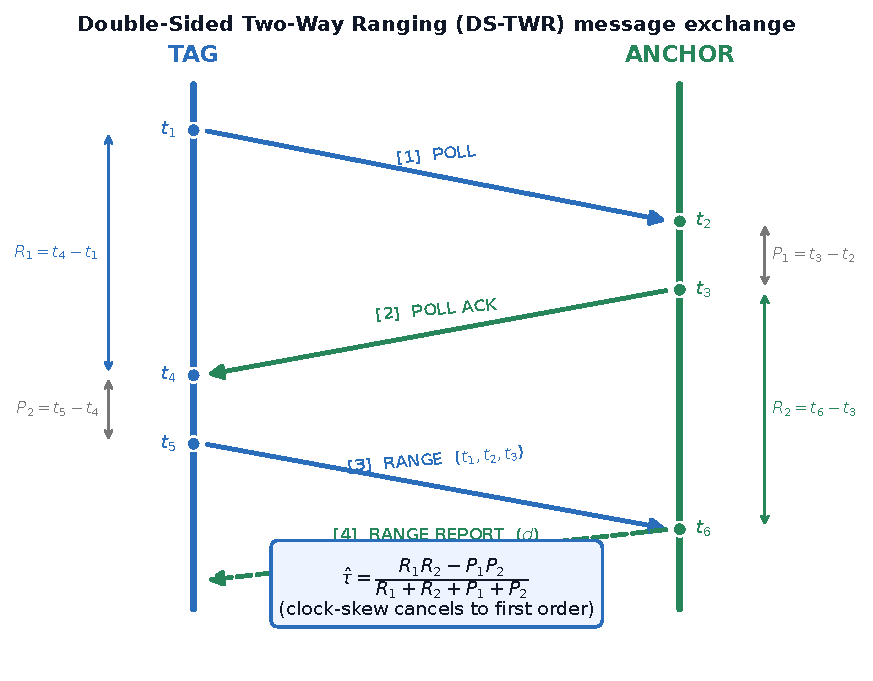
\includegraphics[width=0.92\columnwidth]{figures/dstwr_timing.pdf}
  \caption{DS-TWR four-message exchange.
  Six DW1000 hardware timestamps ($t_1$--$t_6$) are substituted
  into~\eqref{eq:dstwr} to cancel first-order clock-skew.}
  \label{fig:twr_timing}
\end{figure}

\subsection{Frame Format and TDMA Scheduler}
\label{sec:frame_format}

Every UWB payload begins with a 4-byte application header:
\texttt{[type:1B][src:1B][dst:1B][seq:1B]}.
Addressed POLLs ensure only the target anchor replies, eliminating the
broadcast collisions of existing libraries.
Eight message types (Table~\ref{tab:msg_types}) cover ranging,
remote antenna-delay configuration, and anchor self-survey.
Because timestamps are packed into a fixed 15-byte payload independent of
anchor count, the four-anchor buffer limit of prior libraries is removed entirely.

\begin{table}[h]
  \centering
  \caption{UWB application-layer message types.}
  \label{tab:msg_types}
  \begin{tabular}{llc}
    \toprule
    Mnemonic & Function & Code \\
    \midrule
    \texttt{MSG\_POLL}          & Ranging initiation        & 0x01 \\
    \texttt{MSG\_POLL\_ACK}     & Anchor timestamp reply    & 0x02 \\
    \texttt{MSG\_RANGE}         & Tag timestamp transfer    & 0x03 \\
    \texttt{MSG\_RANGE\_REPORT} & Anchor distance report    & 0x04 \\
    \texttt{MSG\_SURVEY\_REQ}   & Anchor self-survey start  & 0x05 \\
    \texttt{MSG\_SURVEY\_RESP}  & Survey range response     & 0x06 \\
    \texttt{MSG\_ANT\_DELAY}    & Remote delay push         & 0x07 \\
    \texttt{MSG\_ANT\_DELAY\_ACK} & Delay acknowledged      & 0x08 \\
    \bottomrule
  \end{tabular}
\end{table}

The tag cycles through $N$ anchors in round-robin order.
If an anchor fails for three consecutive sweeps it is skipped with exponential
back-off (5, 10, 20, 40 sweeps), then retried --- keeping throughput high when
one anchor is temporarily obstructed.
One complete sweep takes $N \times \approx\SI{25}{\milli\second}$,
giving $\approx\SI{10}{\hertz}$ for $N = 4$ active anchors.

\subsection{Comparison with Existing Libraries}
\label{sec:library_comparison}

Table~\ref{tab:library_comparison} compares DUNE against the five most widely
used open-source DW1000 libraries across the five limitations identified in
\S\ref{sec:limitations}.

\begin{table}[h]
  \centering
  \caption{Open-source Decawave DW1000 library comparison.}
  \label{tab:library_comparison}
  \resizebox{\columnwidth}{!}{%
  \begin{tabular}{lcccccc}
    \toprule
    Library & Ceil. & No coll. & Rate (Hz) & Multi-tag & NLOS & Survey \\
    \midrule
    thotro \cite{thotro_dw1000}   & 4 & \texttimes & \todo{} & \texttimes & \texttimes & \texttimes \\
    jremington fork               & 7* & \texttimes & \todo{} & \texttimes & \texttimes & \texttimes \\
    pizzo00 fork                  & 6  & \texttimes & \todo{} & \texttimes & \texttimes & \texttimes \\
    Makerfabs example             & 4  & \texttimes & \todo{} & \texttimes & \texttimes & \texttimes \\
    dw1000-ng                     & \todo{} & \texttimes & \todo{} & \texttimes & \texttimes & \texttimes \\
    \textbf{Ours (DUNE)}          & $\mathbf{N}$ & \checkmark & \textbf{\todo{10}} & \checkmark & \checkmark & \checkmark \\
    \bottomrule
  \end{tabular}}
  \smallskip\par
  *jremington raises \texttt{MAX\_DEVICES} to 7 without fixing the encoding;
  5+ anchors overflows silently.
\end{table}
